\chapter{Analysis and evaluation}\label{cap:analysis}

This chapter presents an analysis of the performance of the chess engine through profiling, identifying its most computationally intensive components. We then describe the testing framework used to evaluate the effectiveness of the optimization techniques introduced in~\cref{cap:ImprovementTechniques}. These evaluations are based on 100-game matches between different versions of the engine and a baseline implementation. Finally, we compare the performance of \textit{AlphaDeepChess} against \textit{Stockfish} and examine its position within the Elo rating distribution on \textit{Lichess.org}.

\section{Profiling}
In order to analyze the performance of our chess engine and identify potential bottlenecks where the code consume the most execution time, we used the \texttt{perf} tool available on Linux systems. \texttt{perf} provides robust profiling capabilities by recording CPU events, sampling function execution, and collecting stack traces~\cite{PerfLinux}. 

\vspace{1em}

\noindent We run the engine under \texttt{perf} using the following commands:

\begin{lstlisting}[language=bash, caption={Profiling \textit{AlphaDeepChess} with perf}, frame=single, breaklines=true]
# Record performance data with function stack traces
sudo perf record -g ./build/release/AlphaDeepChess

# Display interactive report
sudo perf report -g --no-children
\end{lstlisting}

\noindent After recording, \texttt{perf report} opens an interactive terminal interface where functions are sorted by CPU overhead, allowing us to easily identify performance-critical regions.

\vspace{2em}

\noindent First, we profile the basic architecture of the engine implemented in~\cref{cap:descripcionTrabajo}, and then evaluate it again after applying the optimizations described in~\cref{cap:ImprovementTechniques}.

\subsection*{Profiling of basic engine architecture}

\noindent As shown in~\cref{tab:profilingBasic}, the profiling results indicate that the majority of the total execution time is spent in the legal move generation function. Specifically, the functions \texttt{generate\_legal\_moves}, \texttt{calculate\_moves\_in\_dir}, and \texttt{update\_danger\_in\_dir} together account for over 72\% of the total overhead. Therefore, the optimizations on this component are expected to yield significant performance improvements.

\begin{table}[H]
    \centering
    \begin{tabular}{|l|r|}
    \hline
    \textit{Symbol} & \textit{Overhead} \\
    \hline
    \texttt{generate\_legal\_moves}       &  36.07\% \\
    \texttt{calculate\_moves\_in\_dir}    &  19.30\% \\
    \texttt{evaluate\_position}          &  16.63\% \\
    \texttt{update\_danger\_in\_dir}      &   16.23\% \\
    \texttt{calculate\_king\_moves}       &   1.24\% \\
    \texttt{quiescence\_search}          &   0.96\% \\
    \texttt{...}                          &   ...     \\
    \hline
    \end{tabular}
    \caption{Profiling results of the basic engine implementation.}
    \label{tab:profilingBasic}
\end{table}

\vspace{1em}

\subsection*{Profiling with improvement techniques}

\noindent As shown in~\cref{tab:profilingImprovements}, the updated profiling results demonstrate a successful reduction in the computational cost of move generation. The execution time is now more evenly distributed across various modules, with position evaluation emerging as the new primary performance bottleneck. This shift confirms the effectiveness of the implemented optimization techniques.

\begin{table}[H]
    \centering
    \begin{tabular}{|l|r|}
    \hline
    \textit{Symbol} & \textit{Overhead} \\
    \hline
    \texttt{evaluate\_position}       &  31.90\% \\
    \texttt{update\_attacks\_bb}    &  22.62\% \\
    \texttt{generate\_legal\_moves}          &  22.71\% \\
    \texttt{order\_moves}      &   3.95\% \\
    \texttt{make\_move}       &   3.83\% \\
    \texttt{alpha\_beta\_search}          &   1.66\% \\
    \texttt{...}                          &   ...     \\
    \hline
    \end{tabular}
    \caption{Profiling results after applying optimization techniques.}
    \label{tab:profilingImprovements}
\end{table}

\section{Testing framework}

\noindent In this section, we describe the tools used to test and debug the engine, as well as the methodology for evaluating each of the improvement techniques implemented throughout the development of the chess engine.

\subsection*{Graphical user interface}

\noindent Although we implemented a \texttt{diagram} command to display the current position in the standard output, making moves and observing evaluations can be a time-consuming process during debugging and testing. To streamline this workflow, we developed a graphical user interface (GUI) using Python. For rapid development and ease of use, we chose \textit{CustomTkinter}, one of the most widely adopted Python UI libraries.

\vspace{1em}

\parbox{\textwidth}{\noindent The GUI provides a user-friendly interface that communicates with the engine using the UCI protocol under the hood, greatly enhancing the debugging and testing experience. This tool can be used after compiling the engine by running \texttt{AlphaDeepChessGUI.py} with Python.}


\begin{figure}[H]
    \centering
    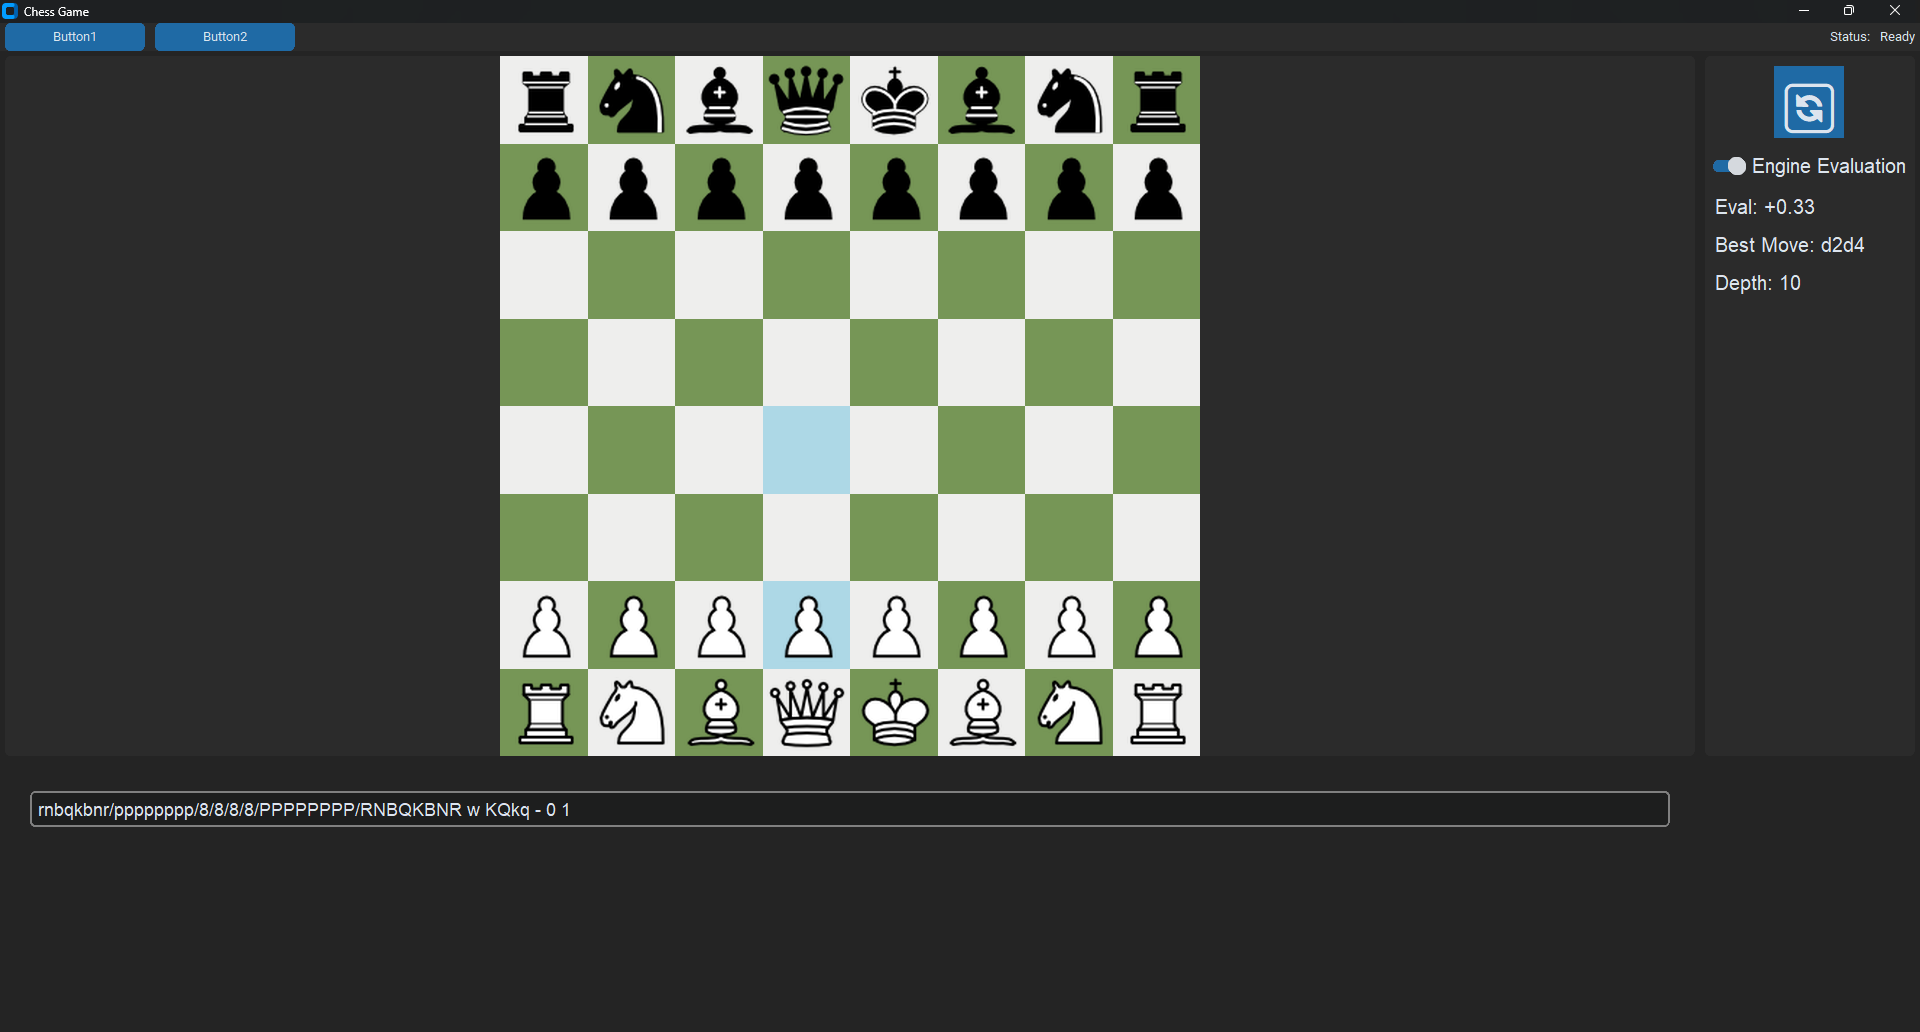
\includegraphics[width=1.0\textwidth]{Imagenes/gui.png}
    \caption{\textit{AlphaDeepChess}'s GUI}\label{fig:gui}
\end{figure}

\noindent In~\cref{fig:gui}, the engine evaluation is enabled and displays the current evaluation value, the best move found, and the calculated search depth. In this way, we also ensure a more user-friendly experience.


\subsection*{\textit{Cutechess}}

\noindent To evaluate the different techniques implemented, we also required a tool capable of running automated tournaments between chess engines. For this task, we used \textit{Cutechess}, whose usage is described in detail in~\cref{sec:cutechess}.

\vspace{1em}

\noindent Depending on the number of games, search time, and time control, these tournaments between engines can take a long time to process. For this reason, we decided to use GitHub Actions and workflows to separate our development environment from the execution of performance and strength tests.

\vspace{1em}

\subsection*{Github actions and workflows}

GitHub Actions is a CI/CD tool integrated into GitHub that allows developers to automate tasks such as building, testing, and deploying code. Workflows are defined in YAML files and specify the tasks to be executed, the jobs or events that trigger them, and the environment in which they run.

\vspace{1em}

\parbox{\textwidth}{\noindent In this project, since it is public in a GitHub repository, we used GitHub Actions to automate the testing and evaluation of the chess engine with \textit{Stockfish} and \textit{Cutechess}. A workflow was configured (located at \texttt{.github\textbackslash{}workflows\textbackslash{}manual-workflow.yml}) to compile the engine and run automated games using \textit{Cutechess} between different versions of the engine or against \textit{Stockfish}.}

\section{Evaluation of improvements}

\noindent In this section we provide the results of a 100-game match between improved engine versions and a baseline version. The purpose of these matches is to measure the improvement in playing strength introduced by each new implementation. All matches are conducted using the tournament manager \textit{Cutechess} with the following configuration:

\begin{enumerate}
    \item 50 unique random starting positions, each played twice with alternating colors.
    \item 4 seconds of thinking time per move.
    \item A 150-move limit per game, after which the game is declared a draw.
\end{enumerate}

\vspace{1em}

\parbox{\textwidth}{The matches were executed on virtual machines provided by \textit{GitHub Actions}, using the ubuntu-latest runner. At the time of testing, this environment provided 4 CPUs, 16 GB of RAM, a 14 GB SSD, and a 64-bit architecture.}

\vspace{1em}

\noindent The baseline engine configuration is shown in~\cref{tab:baselineBot}. It includes only the core techniques described in~\cref{cap:descripcionTrabajo}.

\begin{table}[H]
    \centering
    \begin{tabular}{|p{4cm}|p{4cm}|}
    \hline
    \textit{Component}         & \textit{Baseline Bot}     \\ \hline
    Search                     & Basic Alpha-Beta           \\ \hline
    Evaluation Function        & Materialistic        \\ \hline
    Move Generator             & Basic implementation   \\ \hline
    Move Ordering              & MVV-LVA                \\ \hline
    \end{tabular}
    \caption{Baseline engine configuration.}
    \label{tab:baselineBot}
\end{table}

\subsection*{Transposition table}
\label{sec:tt}

\noindent This experiment evaluates the impact of integrating a transposition table into the search process. The only modification compared to the baseline engine is in the search component.

\vspace{0.5em}

\begin{table}[H]
    \centering
    \begin{tabular}{|p{4cm}|p{6cm}|}
    \hline
    \textit{Component}         & \textit{Engine configuration}            \\ \hline
    Search                     & With Transposition Table \\ \hline
    \end{tabular}
    \caption*{Configuration of Transposition Table Bot.}
    \label{tab:tt_vs_basic}
\end{table}

\begin{center}
\ResultBar{15cm}{0.5cm}{46}{22}{32}
\medskip
\end{center}

\noindent The match results show a clear improvement: 46 wins, 32 losses, and 22 draws. This confirms that transposition tables reduce redundant evaluations and increase search efficiency.

\subsection*{Move generator with magic bitboards and pext instruction}

\noindent In addition to the transposition table, we now accelerate the move generation process using \texttt{PEXT}  instructions. We chose not to analyze the magic bitboards technique at this stage, as both approaches provide constant-time (\( O(1) \)) access to legal moves for sliding pieces, and would yield similar performance results.

\vspace{1em}

\begin{table}[H]
    \centering
    \begin{tabular}{|p{4cm}|p{6cm}|}
    \hline
    \textit{Component}         & \textit{Engine configuration}    \\ \hline
    Search                     & With Transposition Table                     \\ \hline
    Move Generator             & PEXT implementation                \\ \hline
    \end{tabular}
    \caption*{Configuration of PEXT instructions Bot}\label{tab:pext_vs_basic}
\end{table}

\begin{center}
\ResultBar{15cm}{0.5cm}{64}{14}{22}
\medskip
\end{center}

\noindent The results shown a significant performance improvement by adding the PEXT instructions with 46 wins versus 22 losses. The remaining 14 games ended in a draw.

\subsection*{Evaluation with king safety and piece mobility}

\noindent The next step is the introduction of the new parameters in the evaluation.
\vspace{1em}

\begin{table}[H]
    \centering
    \begin{tabular}{|p{4cm}|p{6cm}|}
    \hline
    \textit{Component}         & \textit{Engine configuration}    \\ \hline
    Search                     & With Transposition Table   \\ \hline
    Evaluation Function        & King safety and piece mobility     \\ \hline
    Move Generator             & PEXT implementation                \\ \hline
    \end{tabular}
    \caption*{Configuration of Bot with advanced evaluation parameters.}\label{tab:advancedEval_vs_basic}
\end{table}

\begin{center}
\ResultBar{15cm}{0.5cm}{62}{8}{30}
\medskip
\end{center}

\noindent The results are slightly worse compared to the match using the material-only evaluation shown in the following result bar, with 62 wins and 30 losses. This decline may be attributed to the additional computational overhead introduced by evaluating the new parameters. Moreover, while concepts such as king safety and piece mobility are intuitively valuable to human players, the engine may struggle to consistently associate them with actual positional strength.

\subsection*{Multithreaded search}

\noindent The next experiment evaluated the impact of parallelizing the search. In this setup, the transposition table was disabled due to its inability to handle concurrent access safely in our implementation.

\begin{table}[H]
    \centering
    \begin{tabular}{|p{4cm}|p{6cm}|}
    \hline
    \textit{Component}         & \textit{Engine configuration}         \\ \hline
    Search                     & YBWC Multithreaded Search  \\ \hline
    Move Generator             & PEXT Implementation                \\ \hline
    \end{tabular}
    \caption*{Configuration of the multithreaded bot.}
    \label{tab:multithreadedBot}
\end{table}

\begin{center}
\ResultBar{15cm}{0.5cm}{32}{5}{63}
\medskip
\end{center}

\noindent Despite the theoretical advantage of parallel search, the results showed a decline in performance: 32 wins, 63 losses, and 5 draws. This underperformance may be attributed to several disadvantages of the YBWC algorithm in our implementation, including synchronization overhead, thread creation and destruction costs, and lack of shared transposition table access.

\subsection*{Late move reductions}

\noindent The final technique evaluated is the inclusion of Late Move Reductions (LMR) in the search algorithm. This experiment also includes the transposition table (TT) and the optimized move generator using PEXT instructions.

\begin{table}[H]
    \centering
    \begin{tabular}{|p{4cm}|p{6cm}|}
    \hline
    \textit{Component}         & \textit{Engine configuration}         \\ \hline
    Search                     & with LMR and TT \\ \hline
    Move Generator             & PEXT Implementation                \\ \hline
    \end{tabular}
    \caption*{Configuration of the late move reductions bot.}
    \label{tab:reductionsBot}
\end{table}

\begin{center}
 \ResultBar{15cm}{0.5cm}{48}{15}{37}
\medskip
\end{center}

\noindent The results show 48 wins, 15 draws, and 37 losses. This outcome is slightly worse than the version without reductions. A likely explanation is that the current move ordering heuristic is not strong enough, leading the search to incorrectly reduce important moves that appear late in the move list. As a result, the potential benefits of LMR are not fully realized and may even degrade search quality in some positions.

\vspace{2em}

\noindent We can confirm that \textit{AlphaDeepChess} achieves its maximum skill level with the following configuration:

\begin{table}
    \centering
    \begin{tabular}{|p{4cm}|p{6cm}|}
    \hline
    \textit{Component}         & \textit{Best configuration}         \\ \hline
    Search                     & with Transposition Table    \\ \hline
    Evaluation Function        & Materialistic                          \\ \hline
    Move Generator             & PEXT implementation                    \\ \hline
    Move Ordering              & MVV-LVA                                \\ \hline
    \end{tabular}
    \caption{Best engine configuration.}
    \label{tab:bestEngineConfiguration}
\end{table}


\noindent Now, we compare the skill level of \textit{AlphaDeepChess} with the best configuration against \textit{Stockfish}.

\section{Evaluation versus \textit{Stockfish}}

\begin{center}
 \ResultBar{15cm}{0.5cm}{0}{0}{100}
\medskip
\end{center}

\noindent \textit{AlphaDeepChess} lost all games against \textit{Stockfish}. This outcome was expected, as \textit{Stockfish} has an estimated Elo rating of around 3644~\cite{StockfishElo}, making it orders of magnitude stronger than the best human players. In contrast, as we will show in the next section, \textit{AlphaDeepChess} plays at a level comparable to a strong human player.

\newpage

\section{Engine elo rating in \textit{Lichess}}

\noindent We deployed the engine on \textit{Lichess}, the platform that allows engines to compete against both human players and other bots (see~\cref{sec:lichess}).

\vspace{1em}

\noindent~\cref{fig:eloDistribution} illustrates the Elo rating distribution of players on \textit{Lichess}, where the median rating is approximately 1500.
\vspace{1em}

\noindent After playing more than 500 games, \textit{AlphaDeepChess} achieved an Elo rating of 1900 on \textit{Lichess}~\cite{AlphaDeepChessElo}. This places the engine significantly above the platform's median and within the top percentiles of the player base. For reference, the highest-rated human player on the platform has reached an Elo of 3000 as of 2025~\cite{LichessBestPlayer}.

\begin{figure}
    \centering
    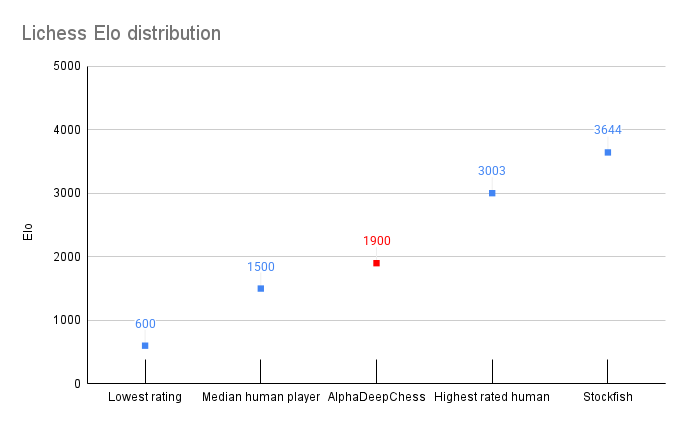
\includegraphics[width=0.95\linewidth]{Imagenes/eloDistribution.png}
    \caption{\textit{Lichess} Elo distribution as of May 2025~\cite{LichessEloDistribution}.}\label{fig:eloDistribution}
\end{figure}